\chapter{Optimierung}
\section{Initialisierung}
Zu Beginn muss die Herde aller Elefanten in Clans aufgeteilt werden, wobei davon ausgegangen wird, dass jeder Clan eine feste Nummer an Tieren beinhaltet. 

\section{Clan-Update-Operator}
\begin{equation}
    x_{new, ci, j} + \alpha \cdot (x_{best, ci} - x_{ci, j}) \cdot r
    \label{calcXNew}
\end{equation}
\begin{equation}
    x_{new, ci, j} = \beta \cdot x_{center, ci}
    \label{calcXNewMatriarch}
\end{equation}

\begin{equation}
    x_{center, ci, d} = \frac{1}{n_{ci}} \cdot \sum_{j=1}^{n_{ci}} x_{ci,j,d}
    \label{calcXCenter}
\end{equation}

\section{Separierungs-Operator}
\begin{equation}
    x_{worst, ci} = x_{min} + (x_{max} - x_{min} + 1) \cdot rand
    \label{calcXWorst}
\end{equation}

\begin{figure}[ht]
    \begin{center}
        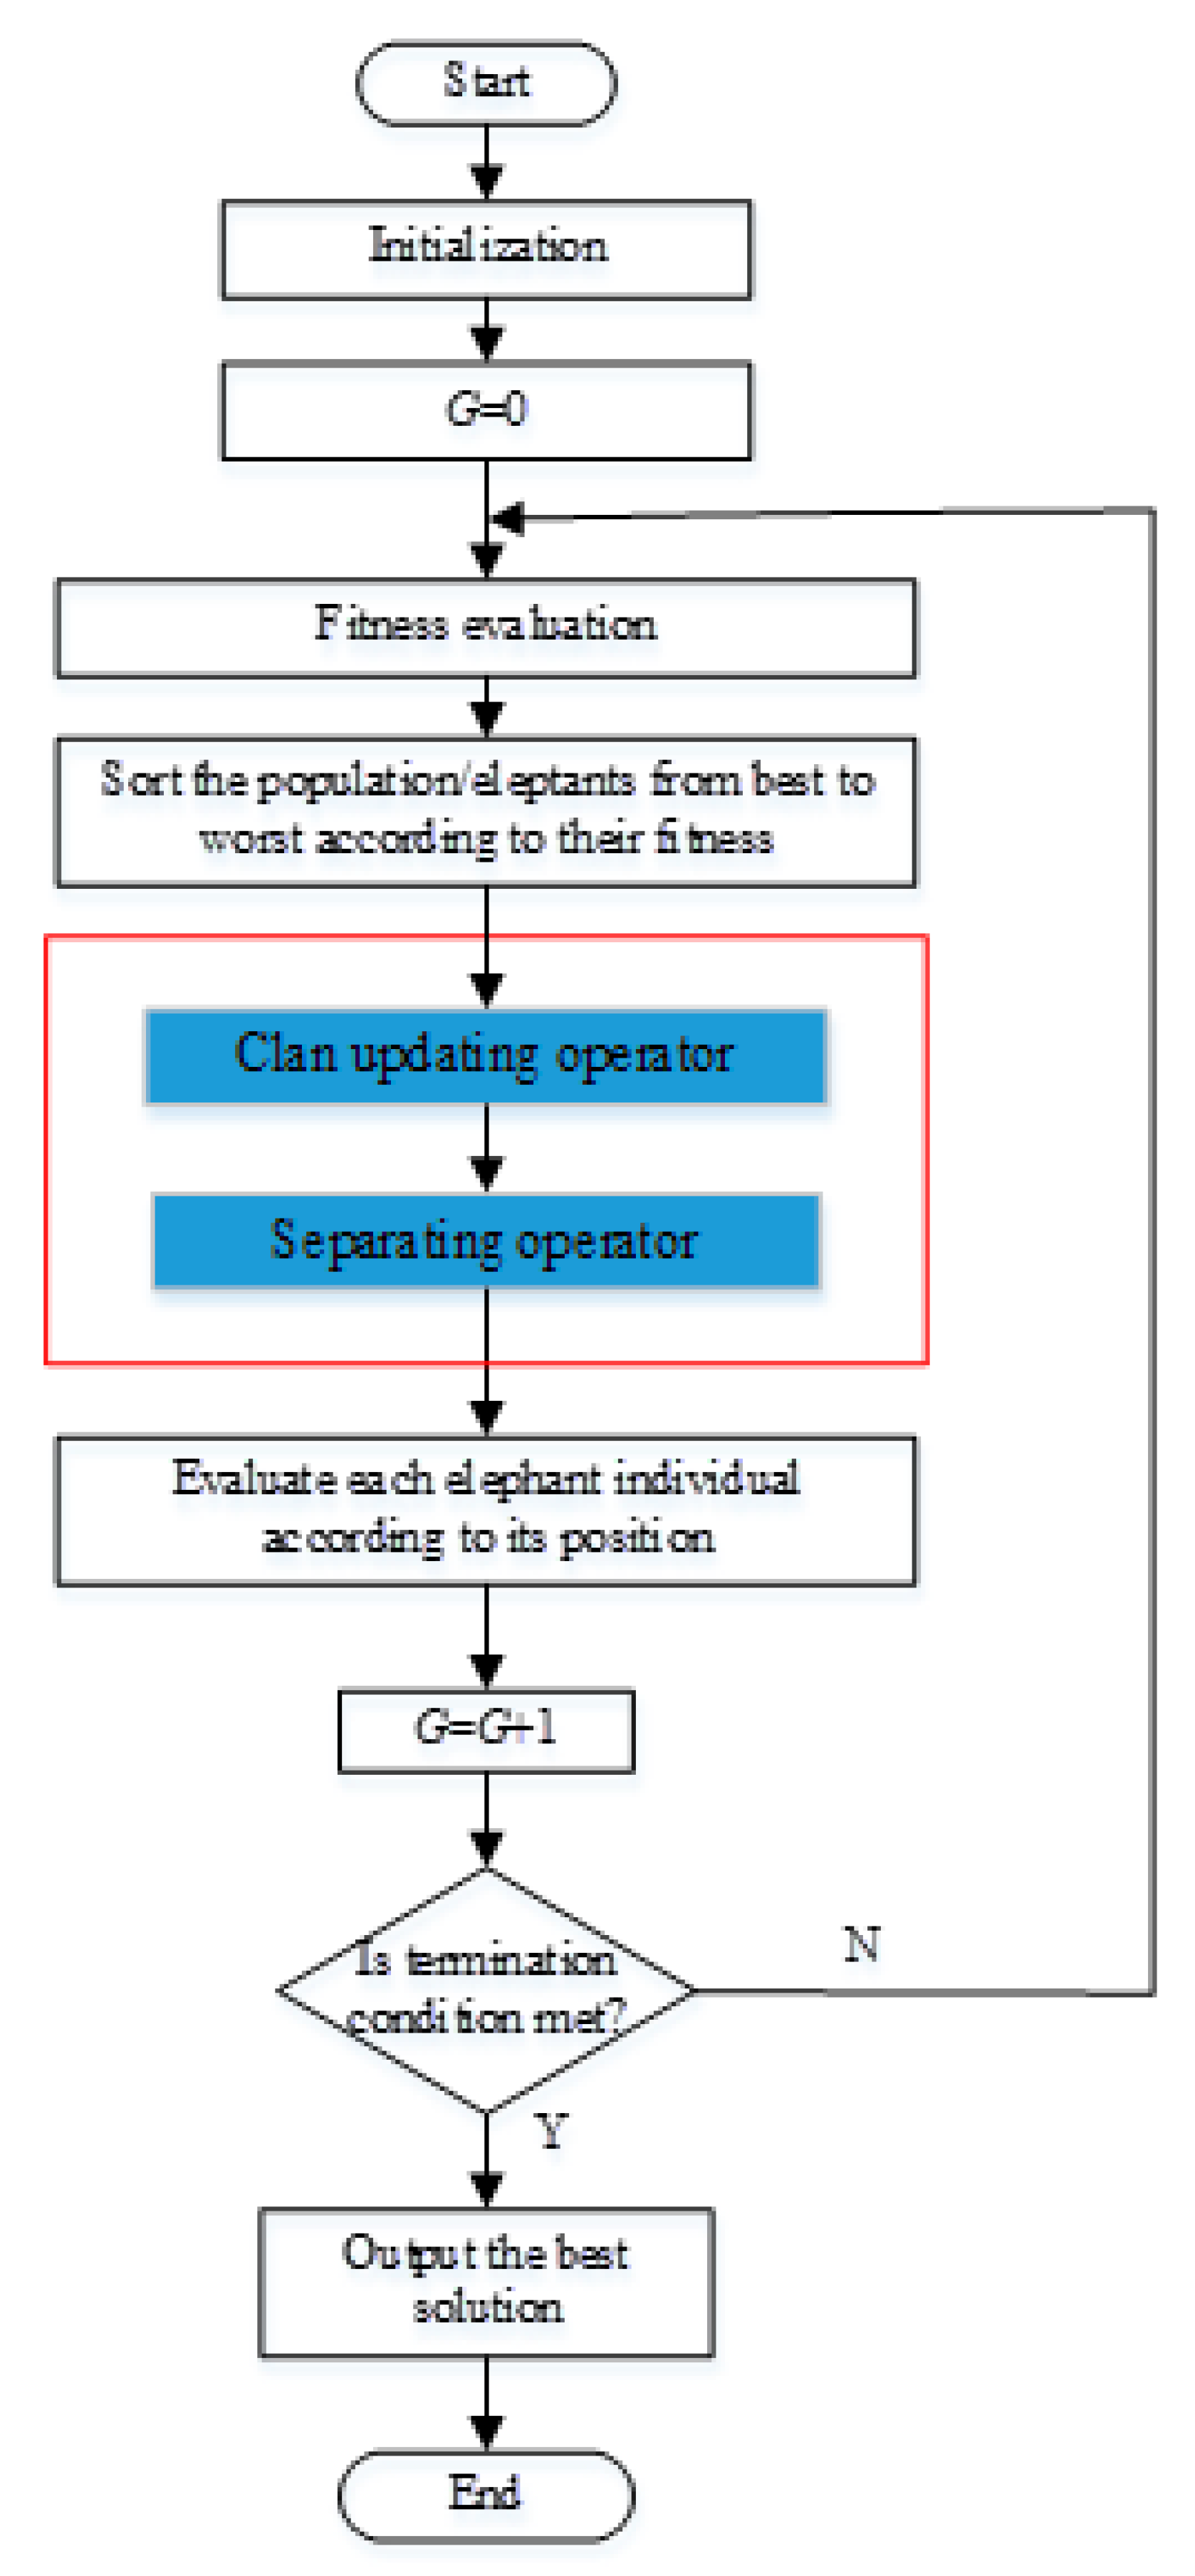
\includegraphics[width=0.5\textwidth]{assets/img/eho_flowchart.png}
        \caption[EHO Flowchart]{\cite[Li et al, S.4]{li_lei_alavi_wang_2020}}
        \label{eho_flowchart}
    \end{center}
\end{figure}

\begin{figure}[ht]
    \begin{center}
        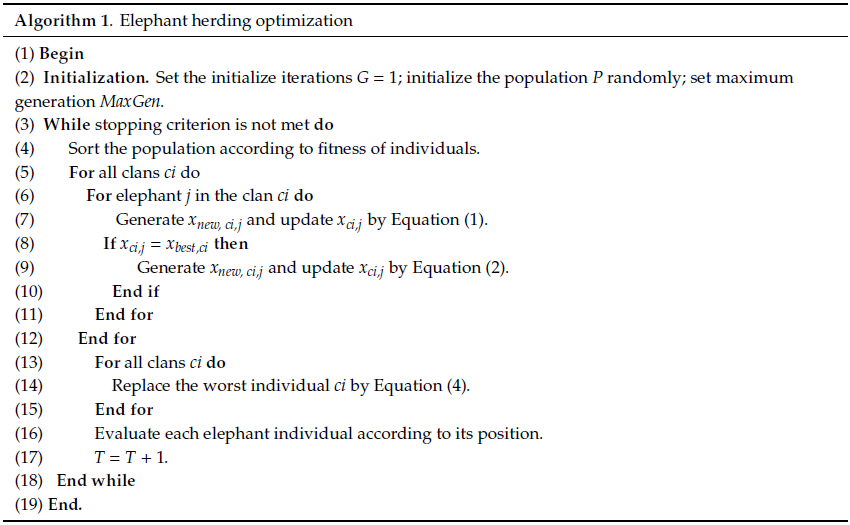
\includegraphics[width=0.9\textwidth]{assets/img/eho_pseudocode.PNG}
        \caption[EHO Pseudocode]{\cite[Li et al, S.5]{li_lei_alavi_wang_2020}}
        \label{eho_pseudocode}
    \end{center}
\end{figure}